\documentclass[11pt,conference]{IEEEtran}

\usepackage{cite}
\usepackage{url}
\usepackage{mathtools}
\usepackage{tikz}

\usetikzlibrary{matrix, fit}
\usetikzlibrary{backgrounds}

\def\BibTeX{{\rm B\kern-.05em{\sc i\kern-.025em b}\kern-.08em
    T\kern-.1667em\lower.7ex\hbox{E}\kern-.125emX}}

% a quote environment with less left indent and no right indent
\newenvironment{myquote}{\list{}{\leftmargin=12pt\rightmargin=0pt}\item[]}{\endlist}

% "tabs" for indenting Alloy statements
\def\TA{\makebox[12pt]{}}
\def\TB{\makebox[24pt]{}}
\def\TC{\makebox[36pt]{}}

% boldface for Alloy keywords
\def\Bopen{\textbf{open} }
\def\Bas{\textbf{as} }
\def\Bsig{\textbf{sig} }
\def\Babstract{\textbf{abstract} }
\def\Bextends{\textbf{extends} }
\def\Bset{\textbf{set} }
\def\Bpred{\textbf{pred} }
\def\Bfact{\textbf{fact} }
\def\Bfun{\textbf{fun} }
\def\Bassert{\textbf{assert} }
\def\Ball{\textbf{all} }
\def\Bsome{\textbf{some} }
\def\Bone{\textbf{one} }
\def\Belse{\textbf{else} }
\def\Bin{\textbf{in} }
\def\Band{\textbf{and} }
\def\Bor{\textbf{or} }
\def\Bnot{\textbf{not} }
\def\Bno{\textbf{no} }
\def\Bimplies{$\Rightarrow$ }
\def\Biff{\textbf{iff} }
\def\Blet{\textbf{let} }
\def\Bseq{\textbf{seq} }

\begin{document}

\title{Sparse}
\author{
  \IEEEauthorblockN{Tristan Dyer}
  \and
  \IEEEauthorblockN{John Baugh}
}

\maketitle

\section{Introduction}

%Computations on sparse matrices are prevalent in scientific and engineering software.  
Sparse matrix data formats are able to compress large matrices with a small number of non-zero elements into a more efficient representation.  
%The development of software that makes use of sparse matrices is a tedious and often error-prone task because of the myriad data formats and complexities involved in tuning the operations on these formats to achieve an efficient implementation.
Scientific and engineering software that make use of sparse matrix formats are often implemented in low-level imperative languages such as C++ and Fortran.  The optimized nature of these software often means that the structural organization of sparse matrix formats and mathematical computations are heavily intertwined.  Additionally, the myriad data formats and complexities involved in tuning the operations on these formats to achieve efficient implementations means that the development of software that makes use of sparse matrices is a tedious and often error-prone task.

Need to add something about how verification of sparse matrix codes is also difficult, and has only really been done by Arnold.  This is one of our major contributions: sparse matrix codes are difficult to verify (see Arnold), and the development of representation invariants for a number of formats can make this easier.  The representation invariants can be directly translated into code, and used during the development and debugging process to verify that operations on matrices never violate the representation invariants (a la Liskov).

A number of approaches have been taken in order to address these issues.  Object-oriented libraries such as PETSc~\cite{petsc2019} and Eigen~\cite{eigenweb2010} provide data abstractions targeted towards specific classes of solvers.  These libraries provide templates that allow developers to assemble sparse matrices without having to address the structural complexities that a specific format may present.  These matrices can then be used in a variety of solvers, given that the format is supported.

Alternatively, there is a body of research that takes the approach of designing and building compilers capable of automatically making decisions about sparse matrix formats and operations.  Some compilers~\cite{bik1995, bik1996} allow developers to work with dense matrices in code, generating a sparse matrix program at compile time.  Others~\cite{kotlyar1997} allow the user to provide the compiler with an abstract description of a sparse format, from which the compiler can make automatic optimizations in code that accesses the sparse data.

We describe an approach that allows developers to reason about the inherent complexities of sparse matrix formats and operations and to determine invariants that can be used to verify implementations.
%Rather than hiding the complexities of sparse matrix formats by providing data abstractions in code or automatic optimizations in compilers, we propose an approach that allows developers to reason about these complexities.  
Elements of this approach include declarative modeling and automatic, push-button analysis using the Alloy Analyzer~\cite{jackson2012}, a lightweight bounded model checking tool.  Characteristics of sparse matrices, with their numerous representations and ...hard-to-get-right-implementation-details... are approached using abstraction based methods~\cite{clarke1994}, including data abstraction~\cite{dingel1995} and predicate abstraction~\cite{graf1997}, data and functional refinement~\cite{woodcock1996}, and other techniques, manually, as part of a modeling process...

The benefits of this approach lie in its generality.  By using Alloy to perform the modeling and analysis, the modeler may choose the programming language that best fits their needs when transitioning from model to implementation.
Can reason about existing software.
Can reason about design of new sparse matrix libraries.
Can reason about compiler design.

\section{Related Work}

Libraries.
Compilers.
Specifying sparse matrix code.
Verifying sparse matrix code.
Higher order verification.

\section{Lightweight Formal Methods}

...
An additional aspect of lightweight formal methods is an incremental style of modeling, which tools like Alloy support by offering immediate feedback while models are being constructed: we start with a minimal set of constraints and ``grow'' them via conjunction.

\subsection{Alloy}

The tool used in our approach is Alloy, a declarative modeling language combining first-order logic with relational calculus and associated quantifiers and operators, along with transitive closure.  It offers rich data modeling features based on class-like structures and an automatic form of analysis that is performed within a bounded scope using a SAT solver.  For \emph{simulation}, the analyzer can be directed to look for instances satisfying a property of interest.  For \emph{checking}, it looks for an instance violating an assertion: a counterexample.  The approach is \emph{scope complete} in the sense that all cases are checked within user-specified bounds.  Alloy's logic supports three distinct styles of expression, that of predicate calculus, navigation expressions, and relational calculus.  The language used for modeling is also used for specifying properties of interest and assertions.  Alloy supports expressions with integer values and basic arithmetic operations.

\subsection{Data Abstraction}

Proof obligations: mathematical formula to be proven in order to ensure that a component is correct.

Start example here.

\subsection{Data Refinement}

The process of data refinement involves removing nondeterminism, or uncertainty, from an abstract model~\cite{woodcock1996}.  While an abstract model may omit certain design choices, a refinement can resolve some of these choices, removing uncertainty and approaching the level of a concrete implementation.

Diagram of refinement here.

Abstraction function and representation invariant discussion.

Continue example with refinement here.

\section{Sparse Matrix Models}

In this section we describe four models.  First we describe an abstract model of a matrix that does not represent any specific data format, leaving out all implementation details and notions of sparsity. Then we describe three refinements of this model that introduce structure that supports a sparse representation: the DOK format, the ELL format, and the Yale format.  In each of these refinements we determine the appropriate representation invariants as well as the abstraction functions and show that the refinement is valid.

By design, Alloy provides no means of working with floating point values.  It includes integers, but in a limited scope, and so they are not useful when attempting to work with the complete integer set, as might be the case when considering values that could be stored in a sparse matrix.  This is inconsequential, however, as we only aim to reason about the structural complexities of sparse matrix formats.  Therefore, it is sufficient to create an abstract distinction between zero and non-zero values.  Our models employ a Value signature, representing any numerical value, and a Zero signature, an extension of Value, that represents the value zero.  Depending on the scope, this creates an abstract set of ``values'' that we can use to populate matrices in our models.

\begin{displaymath}
Value = \{Zero, Value_0, Value_1, \ldots, Value_n\}
\end{displaymath}

\subsection{Abstract Sparse Matrix}

What is the specification we are modeling?  2D matrix of numerical values: zero or more rows, zero or more columns, a numerical value at every row, column index location.

Our abstract model of a matrix, sparse or otherwise, is defined by the Matrix signature, shown in \figurename~\ref{model:abstract}.  There are three fields defined on the Matrix signature representing (1) the number of rows in the matrix, (2) the number of columns in the matrix, and (3) the values and their locations in the matrix.

\begin{figure}
\centering
\begin{myquote}
\Bsig Matrix \{\\
\TA  rows, cols: Int,\\
\TA  values: Int $\rightarrow$ Int $\rightarrow$ Value\\
\}
\end{myquote}
\caption{Abstract Matrix Model.}
\label{model:abstract}
\end{figure}

This model alone is an underspecified representation of a matrix as it allows, e.g. negative values for the number of rows and columns.  We must include a representation invariant, defined as follows, in order to restrict the allowable set of objects to those that adhere to the specification of a two-dimensional matrix.

\begin{itemize}
	\item The number of rows and columns are each greater than or equal to zero
	\item All index values fall within bounds
	\item The total number of values in the matrix is \(nrows \times ncols\)
	\item Every \(i, j\) index pair appears in the matrix
\end{itemize}

This completes our abstract model of a matrix.  It can be used to represent any two-dimensional matrix that contains values.  Being our highest level of abstraction, it makes no assertions about what values may be included in the matrix or how those values must be stored.

Show an instance here, using visualizations from Alloy Instances preferably.

\subsection{DOK Format}

The dictionary of keys (DOK) format makes use of dictionaries, or associative arrays, to store key, value pairs.  An associative array is a collection of key, value pairs in which each possible key may appear only once.  Sparse matrices are stored such that pairs of row, column indices are used as keys to reference stored values.  The DOK format is frequently used~\cite{scipy, eigenweb2010} in the assembly of sparse matrices because of the efficient \(\mathcal{O}(1)\) access to individual elements provided by the associative array format.  However, because associative arrays make no guarantees about memory locality, iterating over all values in the matrix can be inefficient.  As a result, it is common to use this format to incrementally assemble the full matrix and convert it to another sparse matrix format that allows for more efficient operations on matrices.

The DOK signature is almost identical to the Matrix signature.  The \(rows\) field represents the integer number of rows in the matrix and the \(cols\) field represents the integer number of columns in the matrix.  The \(dict\) field represents the dictionary of key, value pairs.  It takes the same form as the values field of the Matrix signature, but the \(Int \to Int\) relation represents integer pairs used as keys in the dictionary.

\begin{figure}
\centering
\begin{myquote}
\Bsig DOK \{\\
\TA  rows, cols: Int,\\
\TA  dict: Int $\rightarrow$ Int $\rightarrow$ Value\\
\}
\end{myquote}
\caption{DOK Model.}
\label{model:dok}
\end{figure}

In order to limit the scope of instances to only those that accurately represent the properties of an associative array that stores a sparse matrix, we have created the following representation invariant:

\begin{itemize}
  \item The integer value \(rows \geq 0\)
  \item The integer value \(cols \geq 0\)
  \item There are no zeros stored as values
  \item All row, column pairs fall within bounds
  \item All row, column pairs may appear only once
\end{itemize}

The abstraction function:

\begin{itemize}
  \item \(nrows\) equal to number of rows in matrix
  \item \(ncols\) equal to number of columns in matrix
  \item All \((i, j), v\) key, value pairs map to corresponding values in the matrix
  \item All \((i, j)\) pairs \emph{not} in DOK map to zeros in the matrix
\end{itemize}

\subsection{ELL Format}

ELL, coming soon.

\subsection{Yale Format}

The Yale, or frequently, Compressed Sparse Row (CSR) format, uses three arrays to store a sparse matrix.  The array $IA$ stores indices into the other two arrays.  Each consecutive pair of indices in the $IA$ array represents the range of values in the other two arrays that store the data for a single row in the matrix.  So, for example, the first two values in the $IA$ array represent the range of values in the other two arrays that contain data for the first row of the matrix.  The $A$ array contains values while the $JA$ array contains the corresponding column in which each value of the $A$ array falls.

\begin{figure}
\centering
% \begin{displaymath}
%   \begin{pmatrix}
%     4 & 0 & 0 & 0 \\
%     0 & 8 & 15 & 0 \\
%     0 & 0 & 16 & 0 \\
%     23 & 0 & 0 & 42
%   \end{pmatrix}
% \end{displaymath}

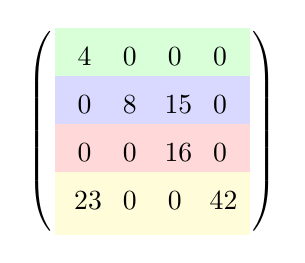
\begin{tikzpicture}
    \matrix[
        matrix of math nodes,
        row sep=.5ex,
        column sep=.5ex,
        left delimiter=(,right delimiter=),
        nodes={text width=.75em, text height=1.5ex, text depth=.5ex, align=center}
        ] (m) 
        {
        4 & 0 & 0 & 0 \\
        0 & 8 & 15 & 0 \\
        0 & 0 & 16 & 0 \\
        23 & 0 & 0 & 42 \\
        };
        \begin{scope}[on background layer]
            \node[fit=(m-1-1)(m-1-4), draw=green!15, fill=green!15] {};
            \node[fit=(m-2-1)(m-2-4), draw=blue!15, fill=blue!15] {};
            \node[fit=(m-3-1)(m-3-4), draw=red!15, fill=red!15] {};
            \node[fit=(m-4-1)(m-4-4), draw=yellow!15, fill=yellow!15] {};
        \end{scope} 
\end{tikzpicture}

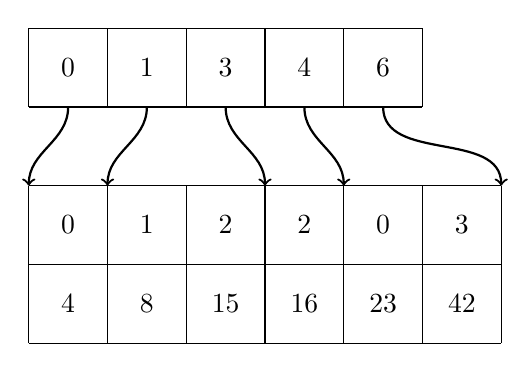
\begin{tikzpicture}
\draw (0,0) grid +(5,1);
\node at (0.5, 0.5) {0};
\node at (1.5, 0.5) {1};
\node at (2.5, 0.5) {3};
\node at (3.5, 0.5) {4};
\node at (4.5, 0.5) {6};

\draw(0,-1) grid +(6,-2);

\node at (0.5, -1.5) {0};
\node at (1.5, -1.5) {1};
\node at (2.5, -1.5) {2};
\node at (3.5, -1.5) {2};
\node at (4.5, -1.5) {0};
\node at (5.5, -1.5) {3};

\node at (0.5, -2.5) {4};
\node at (1.5, -2.5) {8};
\node at (2.5, -2.5) {15};
\node at (3.5, -2.5) {16};
\node at (4.5, -2.5) {23};
\node at (5.5, -2.5) {42};

\draw [thick,->] (0.5,0) to[out=-90, in=90] (0, -1.0);
\draw [thick,->] (1.5,0) to[out=-90, in=90] (1, -1.0);
\draw [thick,->] (2.5,0) to[out=-90, in=90] (3, -1.0);
\draw [thick,->] (3.5,0) to[out=-90, in=90] (4, -1.0);
\draw [thick,->] (4.5,0) to[out=-90, in=90] (6, -1.0);
\end{tikzpicture}

% \begin{displaymath}
%   A = \begin{bmatrix}
%   4 & 8 & 15 & 16 & 23 & 42
%   \end{bmatrix}
% \end{displaymath}
% \begin{displaymath}
%   IA = \begin{bmatrix}
%   0 & 1 & 3 & 4 & 6
%   \end{bmatrix}
% \end{displaymath}
% \begin{displaymath}
%   JA = \begin{bmatrix}
%   0 & 1 & 2 & 2 & 0 & 3
%   \end{bmatrix}
% \end{displaymath}
\end{figure}

Description of where and why it is used... scientific software, good memory locality for sparse matrix-vector multiplication.

\begin{figure}
\centering
\begin{myquote}
\Bsig Yale \{\\
\TA  rows, cols: Int,\\
\TA  A: \Bseq Value,\\
\TA  IA, JA: \Bseq Int,\\
\}
\end{myquote}
\caption{Yale Model.}
\label{model:yale}
\end{figure}

Need to describe the ``get'' predicate and why it is needed.

The abstraction function:

\begin{itemize}
  \item \(nrows\) equal to number of rows in matrix
  \item \(ncols\) equal to number of columns in matrix
  \item For all integers \(i \in [0, nrows)\) and \(j \in [0, ncols)\):
  \begin{itemize}
    \item The value of the ``get'' predicate at \((i, j)\) is equal to the value at location \((i, j)\) in the matrix.
  \end{itemize}
\end{itemize}

The representation invariant:

\begin{itemize}
  \item The integer value \(nrows \geq 0\)
  \item The integer value \(ncols \geq 0\)
	\item There are no zeros stored as values
	\item All values in IA \(\leq nrows \times ncols\)
	\item All values in JA \(< ncols\)
	\item The first value in IA is zero
	\item The last value in IA is the length of A
	\item The last value of IA is not repeated
	\item A and JA are the same length
	\item The max length of A is \(nrows \times ncols\)
	\item The max length of IA is \(nrows + 1\)
	\item The values in IA are monotonically increasing
	\item The difference between any two consecutive values in IA must be \(\leq ncols\)
	\item Values in JA must be unique per row
\end{itemize}

\bibliographystyle{IEEEtran}
\bibliography{IEEEabrv,sparse,mybib}

\end{document}
